\documentclass[]{article}
\pagenumbering{gobble}
\usepackage[a3paper]{geometry}
\usepackage{amsmath, amssymb, amscd, amsthm, amsfonts}
\usepackage{graphicx}
\usepackage{tcolorbox}
\usepackage{hyperref}

\title{TD4: LTE Peak Data Rate and NR Latency}
\author{Gabriel PEREIRA DE CARVALHO}
\date{Last modification: \today}

\begin{document}
	
	\maketitle
	
	\subsection*{Question 1}
	
	The maximum possible signal bandwidth in LTE is $20$MHz corresponding to $100$ resource blocks.
	
	\subsection*{Question 2}
	
	In the normal configuration, LTE has $7$ OFDM symbols per slot.
	
	Each radio frame has $20$ slots $\implies$ $140$ OFDM symbols per radio frame.
	
	Now we do dimensional analysis to get the corresponding number of REs,
	
	\begin{equation}
		1 \text{ radio frame} \cdot \frac{20 \text{ slots}}{1 \text{ radio frame}} \cdot \frac{100 \text{ RBs}}{1 \text{ slot}} \cdot \frac{84 \text{ REs}}{1 \text{ RB}} = 168000 \text{ REs}
	\end{equation}
	
	\subsection*{Question 3}
	
	To maximize the data rate, the control region occupies one OFDM symbol per sub-frame. So the number or REs is
	
	\begin{equation}
		1 \text{ OFDM symbol} \cdot 12 \text{ sub-carriers} \cdot 100 \text{ RBs} = 1200 \text{ REs}
	\end{equation}
	
	% We know that PCFICH is always carried by $16$REs at the first symbol of each subframe (\href{https://sharetechnote.com/html/Handbook_LTE_PCFICH.html}{source}).
	% For PHICH, an ACK or NACK is encoded in 3 bits. Each bit of PHICH is spread by 4 bits using normal prefix $\implies$ each PHICH becomes $12$ bits. PHICH is modulated in BPSK $\implies$ each symbol carries one bit. Each RE carries $1$ symbol $\implies$ we need $12$REs to carry one PHICH (\href{https://sharetechnote.com/html/Handbook_LTE_PHICH_PHICHGroup.html}{source}).
	% The PDCCH occupies the remaining REs in the control region which occupies one symbol per subframe...
	
	\subsection*{Question 4}
	
	The PSS is transmitted in 2 slots per radio frame and mapped to 62 active subcarriers $\implies$ 62 REs per slot. So per frame we have $124$ REs.
	
	Similarly, the SSS is transmitted in 2 slots per radio frame and mapped to 62 active subcarriers $\implies$ 62 REs per slot. So per frame we have $124$ REs.
	
	The PBCH is transmitted in 4 slots per radio frame and mapped to 72 active subcarriers $\implies$ 72 REs per slot. So per frame we have $288$ REs.
	
	In total we have $124 \text{ REs} + 124 \text{ REs} + 288 \text{ REs} = 536 \text{ REs}$.
	
	\subsection*{Question 5}
	
	\begin{figure}[h!]
		\centering
		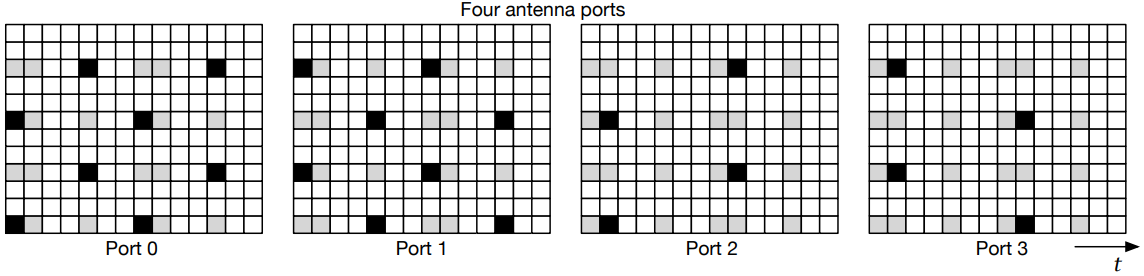
\includegraphics[scale=0.5]{ReferenceSignalsQuestion5.PNG}
		\caption{REs used for Reference signals for 4 antenna transmission}
	\end{figure}
	
	4 antennas $\implies$ 12REs per RB which is $\frac{12}{84} = 14\%$ of all REs.
	
	\subsection*{Question 6}
	
	The densest modulation in LTE is 64-QAM. Each symbol in 64-QAM carries 6 bits.
	
	Maximum number of MIMO parallel flows is 4 (using 4x4 MIMO, 4 input flows/output flows).
	
	Duration of a radio frame is 10ms.
	
	The number of REs transmitting useful data is $168000 \text{ REs} - 1200 \text{ REs} - 536 \text{ REs} = 166264 \text{ REs}$.
	
	Raw peak data rate is
	
	\begin{equation}
		\frac{0.86 \cdot 166264 \text{REs} \cdot 6 \text{bits} \cdot 4 \text{parallel flows}}{10 \text{ms}} = 343.2 \text{Mbps}
	\end{equation}
	
	\subsection*{Question 7}
	
	We have $\frac{3}{4} \cdot 343.2 \text{Mbps} = 257.4 \text{Mbps}$
	
	\subsection*{Question 8}
	
	The measured data rates are probably a bit smaller because we assume ideal channel conditions with no interference, no errors, no congestion and an idealized overhead.
	
	\subsection*{Question 9}
	
	\subsubsection*{OFDM symbol duration}
	
	Without cyclic prefix we have $T_{\text{symbol}} = \frac{1}{\Delta f} = 33.3 \mu s$
	
	With cyclic prefix we have
	
	\begin{align}
		T_{\text{symbol}}^\prime = \frac{1}{\Delta f} + t_{\text{prefix}} = 33.3\mu s + 2.3\mu s = 35.6 \mu s
	\end{align}
	
	\subsubsection*{Duration of the periodic scheme}
	
	We have 3 different periodic schemes: DDDSU, DDDDDDDSUU and DSDU.
	
	The DDDSU scheme has 5 OFDM symbols per period $\implies T_{\text{DDDSU}} = 5 \cdot 35.6 \mu s = 178 \mu s$.
	
	The DDDDDDDSUU scheme has 10 OFDM symbols per period $\implies T_{\text{DDDSU}} = 10 \cdot 35.6 \mu s = 356 \mu s$.
	
	And the DSDU scheme has 4 OFDM symbols per period $\implies T_{\text{DDDSU}} = 4 \cdot 35.6 \mu s = 142.4 \mu s$.
	
	\subsubsection*{Minimum and maximum DL latency}
	
	For minimum latency we consider that reception starts exactly at the beginning of \textbf{S}. For maximal latency, we consider that reception misses the first \textbf{DL} symbol of \textbf{S} and must wait until transmission reaches \textbf{S} again to receive the right data.
	
	\begin{figure}[h!]
		\centering
		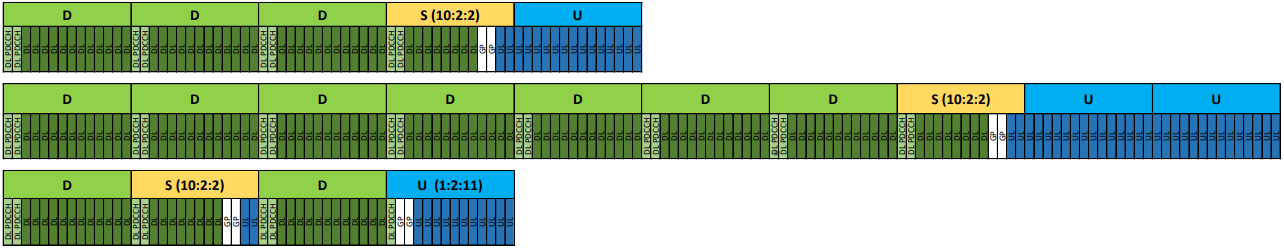
\includegraphics[scale=0.7]{5GframeSchemesQuestion9.PNG}
		\caption{Possible frame structures}
	\end{figure}
	
	\begin{table}[h]
		\centering
		\begin{tabular}{|c|c|c|}
			\hline
			\textbf{Frame Structure} & \textbf{Min DL Latency} & \textbf{Max DL Latency} \\
			\hline
			DDDSU & 12 symbols = 427.2 $\mu$s & 81 symbols = 2883.6 $\mu$s \\
			\hline
			DDDDDDDSUU & 12 symbols = 427.2 $\mu$s & 165 symbols = 5874 $\mu$s \\
			\hline
			DSDU & 12 symbols = 427.2 $\mu$s & 65 symbols = 2314 $\mu$s \\
			\hline
		\end{tabular}
	\end{table}
	
\end{document}